%%%%%%%%%%%%%%%%%%%%%%%%%%%%%%%%%%%%%%%%%%%%%%%%%%%%%%%%%%%%%%%%%%%%
%% I, the copyright holder of this work, release this work into the
%% public domain. This applies worldwide. In some countries this may
%% not be legally possible; if so: I grant anyone the right to use
%% this work for any purpose, without any conditions, unless such
%% conditions are required by law.
%%%%%%%%%%%%%%%%%%%%%%%%%%%%%%%%%%%%%%%%%%%%%%%%%%%%%%%%%%%%%%%%%%%%

\documentclass{beamer}
\usetheme[faculty=ped,basePath=../fibeamer,logo=../fibeamer/logo/mu/Logo-UC-3.png]{fibeamer}
\graphicspath{{../resources/}}

\usepackage{algorithm}
\usepackage{algpseudocode}

\usepackage[utf8]{inputenc}
\usepackage[
  main=english, %% By using `czech` or `slovak` as the main locale
                %% instead of `english`, you can typeset the
                %% presentation in either Czech or Slovak,
                %% respectively.
  czech, slovak %% The additional keys allow foreign texts to be
]{babel}        %% typeset as follows:
%%
%%   \begin{otherlanguage}{czech}   ... \end{otherlanguage}
%%   \begin{otherlanguage}{slovak}  ... \end{otherlanguage}
%%
%% These macros specify information about the presentation
\title{Ejercicos: control de flujo} %% that will be typeset on the
\subtitle{Semestre II-2026} %% title page.
\author{Andreina Cota Vidaurre}
%% These additional packages are used within the document:
\usepackage{ragged2e}  % `\justifying` text
\usepackage{booktabs}  % Tables
\usepackage{tabularx}
\usepackage{tikz}      % Diagrams
\usetikzlibrary{calc, shapes, backgrounds}
\usetikzlibrary{positioning,arrows.meta, shadows.blur}
\usepackage{amsmath, amssymb}
\usepackage{url}       % `\url`s
\usepackage{listings}  % Code listings
\usepackage{graphicx}
\usepackage{amsmath}
\usepackage[T1]{fontenc}
\usepackage{xcolor}
\usepackage{minted}
% \usepackage{adjustbox}


% Definicion de pseudocodigo en espaniol
\lstdefinelanguage{PseudocodigoES}{
    morekeywords={INICIO,FIN,PARA,HACER,SI,ENTONCES,FIN_SI,FIN_PARA,IMPRIMIR},
    sensitive=true,
    morecomment=[l]{//},
    morestring=[b]"
}

% Definicion de pseudocodigo en ingles
\lstdefinelanguage{PseudocodeEN}{
    morekeywords={BEGIN,END,FOR,DO,IF,THEN,END_IF,END_FOR,PRINT},
    sensitive=true,
    morecomment=[l]{//},
    morestring=[b]"
}

\lstset{
    basicstyle=\ttfamily\small,
    keywordstyle=\bfseries,
    columns=fullflexible,
    keepspaces=true,
    showstringspaces=false,
    frame=single,
    xleftmargin=0em,
    framexleftmargin=0em,
    framesep=2pt,
    gobble=4,
    resetmargins=true,
    aboveskip=0pt,
    belowskip=0pt
}

\lstdefinestyle{pythonstyle}{
    language=Python,
    basicstyle=\ttfamily\small,
    keywordstyle=\bfseries,
    commentstyle=\itshape,
    stringstyle=\ttfamily,
    showstringspaces=false,
    columns=fullflexible,
    keepspaces=true,
    frame=single,
    breaklines=true,
    xleftmargin=0em,
    framexleftmargin=0em,
    framesep=2pt,
    aboveskip=0pt,
    belowskip=0pt,
    gobble=4,
    resetmargins=true,
    emph={print,input,int,float,str,bool,len,range},
    emphstyle=\bfseries
}

\lstset{style=pythonstyle}

% \newcolumntype{Y}{>{\raggedright\arraybackslash}X}

\frenchspacing
\begin{document}
  \shorthandoff{-}
  \frame[c]{\maketitle}


    \begin{frame}{1. Extinción de los dinosaurios}
        Hace aproximadamente 66 millones de años, un gran asteroide impacto la Tierra 
        cerca de la actual peninsula de Yucatán. Este evento está asociado con la extinción 
        masiva que eliminó a gran parte de las especies del planeta, incluidos los dinosaurios no avianos.
        \begin{figure}
            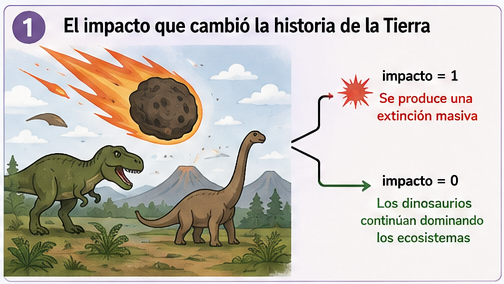
\includegraphics[width=0.7\textwidth]{e1_1.png}
            % \caption{Asteroide que impacto la Tierra}
        \end{figure}
    \end{frame}

    \begin{frame}{1. Extinción de los dinosaurios}
        Una simulación utiliza la variable \mintinline{python}{impacto} donde:
        \begin{itemize}
            \item $1$ (uno) representa que el asteroide impacta la Tierra
            \item $0$ (cero) representa que el asteroide no impacta la Tierra
        \end{itemize}
        Desarrolla un programa que solicite el valor de \mintinline{python}{impacto}.
        
        Si ocurre el impacto, el programa debe mostrar:
        \mintinline{python}{"Se produce una extinción masiva"}

        En caso contrario, debe mostrar:
        \mintinline{python}{"Los dinosaurios continuan vivos"}
    \end{frame}

    \begin{frame}{2. ¿Homo habilis o Homo sapiens?}
        La evolución humana comprende diferentes especies del género Homo. 
        \textit{Homo habilis} apareció mucho antes que \textit{Homo sapiens}.

        En una representación simplificada se utiliza la antigüedad de un fósil 
        expresada en miles de años.

        \begin{figure}
            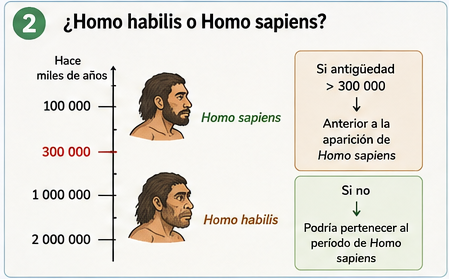
\includegraphics[width=0.7\textwidth]{e2_1.png}
        \end{figure}
    \end{frame}

    \begin{frame}{2. ¿Homo habilis o Homo sapiens?}
        Si el fósil tiene una antigüedad superior a 300000 años, el programa debe mostrar:
        \mintinline{python}{"El fosil es anterior a la aparición de Homo sapiens"}

        En caso contrario, debe mostrar:
        \mintinline{python}{"El fosil podría pertenecer al periodo de Homo sapiens"}
        
    \end{frame}

    \begin{frame}{3. Altura}
        Medida que aumenta la altitud sobre el nivel del mar, disminuye la presión atmosférica y 
        también la disponibilidad de oxígeno para el organismo.

        Un grupo de estudiantes realiza una expedición y quiere generar una advertencia 
        simplificada cuando supera los 2500 m sobre el nivel del mar.

        \begin{figure}
            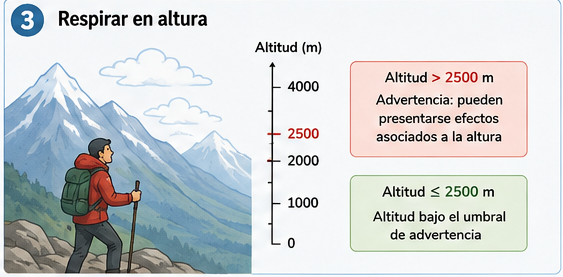
\includegraphics[width=0.7\textwidth]{e3_1.png}
        \end{figure}
    \end{frame}

    \begin{frame}[fragile, t]{3. Altura}
        Realiza un programa que solicite la altitud. Si es mayor que 2500 m, mostrar:
        \begin{minted}{python}
        """Advertencia: pueden presentarse efectos
        asociados a la altura (hipoxia, mareos, etc.)"""
        \end{minted}

        En caso contrario, debe mostrar:
        \begin{minted}{python}
        "Altitud bajo el umbral de advertencia"
        \end{minted}
    \end{frame}

    \begin{frame}{4. Caída libre en otro planeta}
        La aceleracion gravitacional no es igual en todos los cuerpos celestes. Aproximadamente:
        \begin{itemize}
            \item Tierra: 9.81 m/s$^2$
            \item Marte: 3.71 m/s$^2$
        \end{itemize}
        Para una aproximación simple, la velocidad alcanzada después de un tiempo $t$, partiendo del reposo, 
        puede calcularse mediante: $v = g \cdot t$

        \begin{figure}
            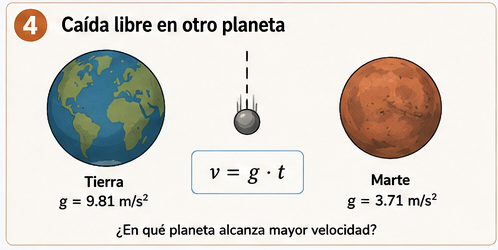
\includegraphics[width=0.7\textwidth]{e4_1.png}
        \end{figure}
    \end{frame}

    \begin{frame}{4. Caída libre en otro planeta}
        Solicita el tiempo de caída de un objeto en segundos y calcula su velocidad tanto en la Tierra como en Marte.
        
        Luego muestra en qué planeta alcanza una mayor velocidad.
    \end{frame}

    \begin{frame}{5. Energía cinética de un vehículo}
        La energía cinética depende de la masa y de la velocidad:

        $E_k = \frac{1}{2} m v^2$ donde $m$ es la masa y $v$ es la velocidad.

        Una prueba de seguridad considera que una energía superior a 500000 J requiere aplicar medidas adicionales de protección.

        \begin{figure}
            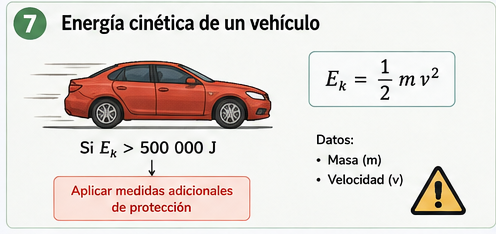
\includegraphics[width=0.7\textwidth]{e5_1.png}
        \end{figure}

    \end{frame}

    \begin{frame}{5. Energía cinética de un vehículo}
        Solicita:

        \begin{itemize}
            \item masa del vehículo en kg;
            \item velocidad en m/s.
        \end{itemize}

        Calcula la energía cinética y determina si supera el umbral.
    \end{frame}

    \begin{frame}{6. Crecimiento poblacional bacteriano}
        En un modelo extremadamente simplificado, una colonia bacteriana duplica su poblacion despues de cada ciclo:

        $N = N_0 \cdot 2^c$ donde:
        \begin{itemize}
            \item $N_0$ es la población inicial;
            \item $c$ es la cantidad de ciclos.
        \end{itemize}

        \begin{figure}
            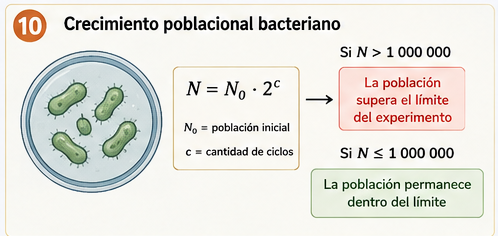
\includegraphics[width=0.7\textwidth]{e6_1.png}
        \end{figure}
    \end{frame}

    \begin{frame}{6. Crecimiento poblacional bacteriano}
        Solicita ambos valores y calcula la población final.

        Si supera 1000000 de bacterias, mostrar:
        \mintinline{python}{"Población crítica: N > 1000000"}

        En caso contrario, debe mostrar:
        \mintinline{python}{"Población dentro de los límites"}
    \end{frame}

    \begin{frame}{7. Conversión}
        En topografía, astronomía y sistemas de posicionamiento, 
        los ángulos pueden expresarse en grados, minutos y segundos de arco. 
        Se cumple que: $1^\circ = 60'$ y $1' = 60''$. Por lo tanto:
        $1^\circ = 3600''$

        Un instrumento entrega una medición angular solamente en segundos de arco.
        Desarrolla un programa que solicite la cantidad total de segundos y la 
        transforme a grados, minutos y segundos.

        \begin{figure}
            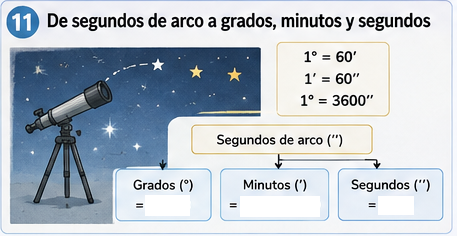
\includegraphics[width=0.7\textwidth]{e7_1.png}
        \end{figure}
    \end{frame}

    \begin{frame}{7. Conversión}
        Por ejemplo, para una medición de 10000 segundos de arco, el 
        programa debe mostrar la cantidad correspondiente de grados, minutos y segundos:
        \mintinline{python}{"2°46'40''"}
    \end{frame} 

    \begin{frame}{8. Sistema rotatorio}
        En mecánica, un eje puede girar varias revoluciones durante su funcionamiento. 
        Una vuelta completa corresponde a: $360^\circ$ 

        Un sensor registra el ángulo total recorrido por un eje, que puede ser mayor que $360^\circ$.

        \begin{figure}
            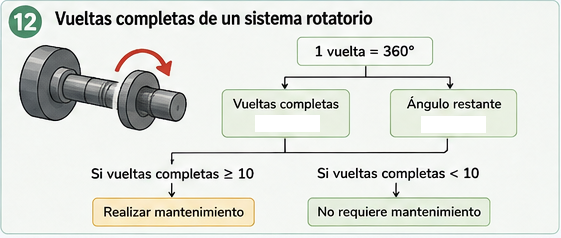
\includegraphics[width=0.7\textwidth]{e8_1.png}
        \end{figure}
    
    \end{frame}

    \begin{frame}{8. Sistema rotatorio}
        Desarrolla un programa que solicite el ángulo total recorrido y calcule:

        \begin{itemize}
            \item el número de vueltas completas;
            \item el ángulo restante.
        \end{itemize}

        \textbf{Desafío adicional:}  Agrega una condición que determine si el sistema requiere 
        mantenimiento. Si el número de vueltas completas es mayor a 10, el programa debe indicar 
        que corresponde realizar mantenimiento. En caso contrario, debe indicar que el sistema puede 
        continuar operando.
    \end{frame}

\end{document}
